\subsection{Computergestützte Analog-zu-Digital-Wandlung} % (fold)
\label{sub:Computergestützte_Analog-zu-Digital-Wandlung}

\begin{frame}
    \frametitle{Computergestützter DAC}
    \framesubtitle{}
     \begin{figure}[H]
     \begin{center}
             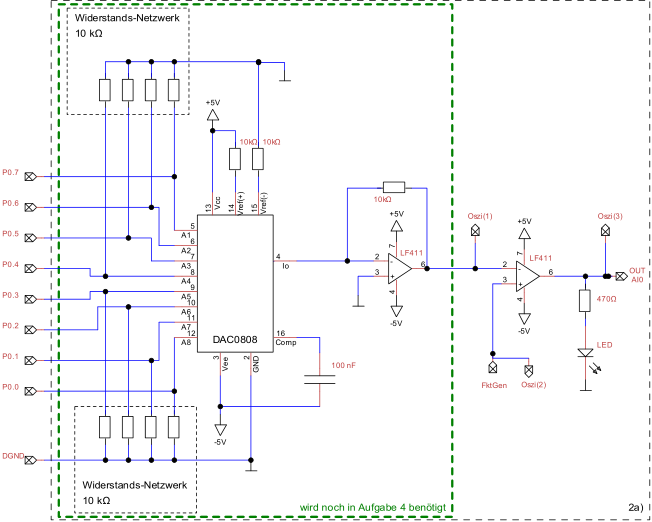
\includegraphics[scale=0.4]{./img/schaltung/comp_dac_0.png}
     \end{center}
     \end{figure}
\end{frame}

\begin{frame}
    \frametitle{Vergleich}
    \framesubtitle{}
    \begin{columns}[c]
        \column{0.5\textwidth}
            \begin{figure}[H]
            \begin{center}
                    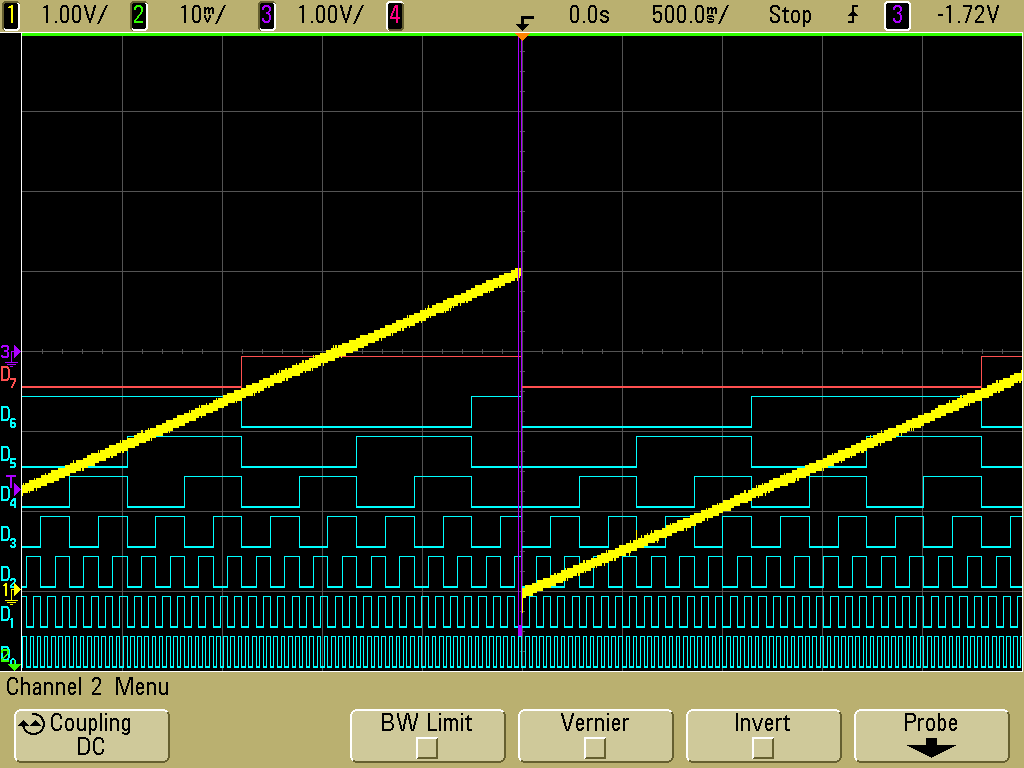
\includegraphics[scale=0.15]{./img/oszi/scope_5.png}
            \end{center}
            \caption{Zählverfahren}
            \end{figure}
        \column{0.5\textwidth}
            \begin{figure}[H]
            \begin{center}
                    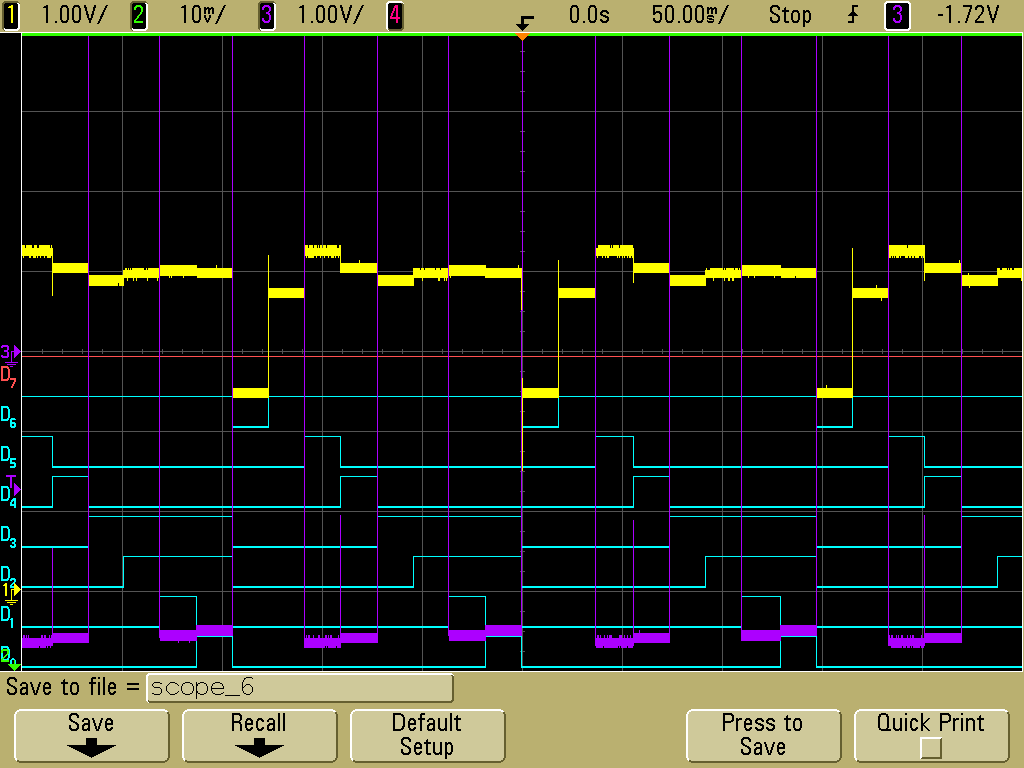
\includegraphics[scale=0.15]{./img/oszi/scope_6.png}
            \end{center}
            \caption{Sukzessive Approximation}
            \end{figure}
    \end{columns}
\end{frame}
\begin{frame}
    \frametitle{Vergleich}
    \framesubtitle{}
    \begin{block}{Vergleich}
        \begin{itemize}
            \item Komplexität beim Zählverfahren steigt mit $2^n$ ($n$: Anzahl
            der Bits)
            \item Komplexität bei sukzessiver Approximation steigt mit $n$
            \item $\rightarrow$ Sukzessive Approximation ist fast immer schneller
            \item Zählverfahren ist schneller falls $U_{analog} < 8 \cdot
            U_{LSB}$
        \end{itemize}
    \end{block}
\end{frame}
\begin{frame}
    \frametitle{Vergleich}
    \framesubtitle{}
    \begin{block}{Störungen}
        Die Spannung wird während der Approximation auf $U_{neu}$ geändert
         \begin{itemize}
             \item Zählverfahren:
             \begin{itemize}
                 \item ist $U_{neu} < U_{Zaehl}$ wird das Verfahren abgebrochen
                 \item ist $U_{neu} > U_{Zaehl}$ wird bis $U_{neu}$
                 weitergezählt
             \end{itemize}
             \item Sukzessive Approximation:
             \begin{itemize}
                 \item ist $U_{neu} < U_{SApr}$ bleiben alle gesetzten Bits
                 bestehem, alle restlichen Bits werden auf 0 gesetzt
                 \item ist $U_{neu} > U_{SApr}$ wird bis $U_{neu}$ fortgesetzt
             \end{itemize}
             \item relevant falls sich Referenzspannung schneller als
             Abtastrate verändert
         \end{itemize}
    \end{block}
\end{frame}

% subsection Computergestützte Analog-zu-Digital-Wandlung (end)
